\documentclass[11pt]{article}

% Basic packages
\usepackage[utf8]{inputenc}
\usepackage[margin=1in]{geometry}
\usepackage{amsmath}
\usepackage{amsfonts}
\usepackage{amssymb}
\usepackage{tikz}

% Document information
\title{Homework 4 - Invariant and Equivariant Neural
Networks}
\author{Ido Nutov \& Tuvy Lemberg}
\date{\today}

\begin{document}

\maketitle

\section{Character inner products and Burnside's lemma}
\label{sec:q1}

We derived all permutation equivariant layers from a vector space $\mathbb{R}^n$ to itself in two seemingly unrelated ways:

\begin{enumerate}
    \item Finding the $S_n$-orbits in $X^2$ where $X = \{1, 2, \ldots, n\}$ and using them to construct equivariant linear maps.
    \item Finding the irreducible subrepresentations of the permutation representation acting on $\mathbb{R}^n$ and then using Schur's Lemma to find all $S_n$-homomorphisms between the irreducible spaces of $\mathbb{R}^n$.
\end{enumerate}

\textbf{Problem.} Use the analysis in Tutorial 12 to prove that these two methodologies both find the number of $G$-equivariant layers from $\mathbb{R}^n$ to $\mathbb{R}^n$ for any finite subgroup $G$ and natural $n$.

\textbf{Solution.}

Let $G \leq S_n$ be a finite subgroup. We want to count the number of $G$-equivariant linear maps $L: \mathbb{R}^n \to \mathbb{R}^n$.

\paragraph{1. Orbit Method (Combinatorial Approach)}

$G$ acts on $X = \{1,2,\ldots,n\}$, and thus on pairs $(i,j) \in X^2$. A linear map $L$ is $G$-equivariant if and only if its matrix $A$ satisfies $A_{g(i),g(j)} = A_{i,j}$ for all $g \in G$. Thus, $A$ is constant on $G$-orbits in $X^2$. The number of independent $G$-equivariant linear maps equals the number of $G$-orbits in $X^2$.

By \textbf{Burnside's Lemma}, the number of orbits is:
\[
\frac{1}{|G|} \sum_{g \in G} |\mathrm{Fix}(g)|,
\]
where $|\mathrm{Fix}(g)|$ is the number of pairs $(i,j)$ fixed by $g$.

\paragraph{2. Representation-Theoretic Method}

The permutation representation of $G$ on $\mathbb{R}^n$ decomposes into irreducible subrepresentations. By Schur's Lemma, the space of $G$-equivariant linear maps is isomorphic to the sum of homomorphism spaces between irreducible components. The dimension of the space of $G$-equivariant maps is:
\[
\sum_{\lambda} (\text{multiplicity of } V_\lambda)^2,
\]
where $V_\lambda$ runs over irreducible representations of $G$ in $\mathbb{R}^n$.

This can also be computed using characters:
\[
\frac{1}{|G|} \sum_{g \in G} \chi(g)^2,
\]
where $\chi$ is the character of the permutation representation (i.e., the number of fixed points of $g$).

\paragraph{3. Equivalence via Burnside's Lemma}

In the orbit method, $|\mathrm{Fix}(g)|$ is the number of pairs $(i,j)$ such that $g \cdot i = i$ and $g \cdot j = j$, i.e., $(\text{number of fixed points of } g)^2$. The character $\chi(g)$ is exactly the number of fixed points of $g$. Therefore,
\[
|\mathrm{Fix}(g)| = (\chi(g))^2.
\]
Thus, both methods yield:
\[
\frac{1}{|G|} \sum_{g \in G} (\chi(g))^2.
\]

\textbf{Conclusion:} Both the orbit method and the representation-theoretic method yield the same formula for the number of $G$-equivariant linear maps from $\mathbb{R}^n$ to itself for any finite subgroup $G \leq S_n$ and any $n$.

\subsection*{Explanation}
Let $G \leq S_n$ be a finite permutation group acting on $n$ elements, and let $\mathbb{R}^n$ be the $n$-dimensional real vector space. We are interested in the space of $G$-equivariant linear maps from $\mathbb{R}^n$ to $\mathbb{R}^n$.

There are two perspectives to count the dimension of this space:

\begin{enumerate}
    \item \textbf{Orbit method:} The group $G$ acts on the set of pairs $(i, j)$, corresponding to the entries of $n \times n$ matrices. The number of $G$-orbits in $X^2$ (where $X = \{1, \ldots, n\}$) equals the number of independent $G$-equivariant linear maps. By Burnside's Lemma, this is given by:
    \[
    \frac{1}{|G|} \sum_{g \in G} (\chi(g))^2,
    \]
    where $\chi(g)$ is the number of fixed points of $g$ in $X$.
    \item \textbf{Representation-theoretic method:} The permutation representation of $G$ on $\mathbb{R}^n$ decomposes into irreducible representations. By Schur's Lemma, the dimension of the space of $G$-equivariant maps is the sum of the squares of the multiplicities of the irreducible components:
    \[
    \sum_{\lambda} (\text{multiplicity of } V_\lambda)^2,
    \]
    where $V_\lambda$ runs over the irreducible representations of $G$ in $\mathbb{R}^n$.
\end{enumerate}

\textbf{Connection:} Both approaches yield the same result because the number of $G$-orbits in $X^2$ is equal to the sum of the squares of the multiplicities of the irreducible representations in the decomposition of $\mathbb{R}^n$. This is a consequence of the fact that the number of $G$-equivariant linear maps is both the number of orbits (by combinatorics) and the sum of squared multiplicities (by representation theory). The equality is made explicit by Burnside's Lemma and the character inner product formula.


\section{Netflix Rating Matrices and Group Equivariance}

\subsection{~}
\subsection{~}
\subsection{~}
\subsection{~}
\subsection{~}


\section{Implementing set networks}

\subsection{~}
\subsection{~}
\subsection{~}
\subsection{~}
\subsection{~}

\section{ Benchmarking Permutation Invariant Networks on 3D Shape Classification}

\subsection{~}
\subsection{~}
\subsection{~}
\subsection{~}
\subsection{~}


\section{Permutation}

Consider the group $S_n \times S_m$, where $S_n$ acts on the rows and $S_m$ acts on the columns of a matrix $A \in \mathbb{R}^{n \times m}$. Let $A$ be a matrix with entries $A_{i,j}$, $1 \leq i \leq n$, $1 \leq j \leq m$.

The vectorization of $A$, denoted $\mathrm{vec}(A)$, is the column vector in $\mathbb{R}^{nm}$ formed by stacking the columns of $A$:
\[
\mathrm{vec}(A) = (A_{1,1}, A_{2,1}, \ldots, A_{n,1}, A_{1,2}, \ldots, A_{n,m})^T
\]

Let $(\sigma, \tau) \in S_n \times S_m$ be a group element, where $\sigma$ permutes the rows and $\tau$ permutes the columns. The action on $A$ is:
\[
A'_{i,j} = A_{\sigma^{-1}(i),\tau^{-1}(j)}
\]

The action on $\mathrm{vec}(A)$ is as follows:
For each entry $A_{i,j}$ in $A$, its position in $\mathrm{vec}(A)$ is $k = n(j-1) + i$.
Under $(\sigma, \tau)$, the entry $A_{i,j}$ moves to the position corresponding to $A_{\sigma(i),\tau(j)}$, which is $k' = n(\tau(j)-1) + \sigma(i)$.

Therefore, the permutation matrix $P_{(\sigma,\tau)}$ acting on $\mathrm{vec}(A)$ is defined by:
\[
P_{(\sigma,\tau)}\mathrm{vec}(A) = \mathrm{vec}(A')
\]
where $A'_{i,j} = A_{\sigma^{-1}(i),\tau^{-1}(j)}$ and the mapping of indices is:
\[
k' = n(\tau(j)-1) + \sigma(i)
\]
for each $k = n(j-1) + i$.

This describes how an element of $S_n \times S_m$ acts on the vectorized matrix.

\subsection*{Parameter Sharing Scheme for Linear Equivariant Layer}

The parameter sharing scheme for a linear $S_n$-equivariant layer (permutation equivariant) can be visualized as follows:


\begin{center}
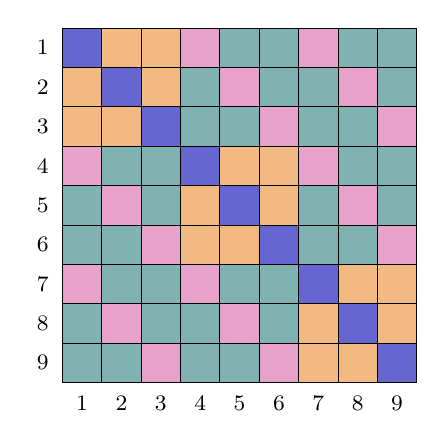
\begin{tikzpicture}[scale=0.5]
    \def\nm{9}
    \def\n{3} % Number of rows
    \def\m{3} % Number of columns
    % Draw the grid and fill colors
    \foreach \ik in {1,...,\n} {
        \foreach \jk in {1,...,\m} {
            \foreach \il in {1,...,\n} {
                \foreach \jl in {1,...,\m} {
                    % Compute the indices
                    \pgfmathsetmacro{\k}{int(\ik + (\jk-1)*\n)}
                    \pgfmathsetmacro{\l}{int(\il + (\jl-1)*\n)}
                    % Color according to orbit type
                    \ifnum\ik=\il
                        \ifnum\jk=\jl
                            % Diagonal within same block: blue
                            \fill[blue!70!black!60] (\l,-\k) rectangle ++(1,1);
                        \else
                            % Diagonal across different blocks: magenta
                            \fill[magenta!80!black!40] (\l,-\k) rectangle ++(1,1);
                        \fi
                    \else
                        \ifnum\jk=\jl
                            % Off-diagonal within same block: orange
                            \fill[orange!90!black!50] (\l,-\k) rectangle ++(1,1);
                        \else
                            % Off-diagonal across different blocks: green
                            \fill[teal!80!black!50] (\l,-\k) rectangle ++(1,1); 
                        \fi
                    \fi
                    \draw[black, line width=0.3pt] (\l,-\k) rectangle ++(1,1);
                }
            }
        }
    }
    % Row and column labels
    \foreach \i in {1,...,\nm} {
        \node[left, font=\footnotesize] at (0.9,{-\i+0.5}) {\i};
        \node[below, font=\footnotesize] at (\i+0.5,-0.1 -\nm) {\i};
    }
\end{tikzpicture}
\end{center}

\noindent
In this scheme, all diagonal elements share the same parameter $a$, and all off-diagonal elements share the parameter $b$. This parameter tying ensures equivariance to permutations of the input.

\section{Orbits under Conjugation Action}

Let $g \in S_{nm}$ be the permutation induced by vectorizing the action of $(\sigma, \tau) \in S_n \times S_m$ on matrices $A \in \mathbb{R}^{n \times m}$. We want to analyze the orbits of the conjugation action $g W g^{-1}$ where $W$ is an $nm \times nm$ matrix.

\subsection{Setup and Notation}

Given $(\sigma, \tau) \in S_n \times S_m$, the induced permutation $g$ on $\mathbb{R}^{nm}$ acts on the vectorized matrix $\mathrm{vec}(A)$ by:
\[
g \cdot \mathrm{vec}(A) = \mathrm{vec}((\sigma, \tau) \cdot A)
\]

The conjugation action on matrices $W \in \mathbb{R}^{nm \times nm}$ is:
\[
W \mapsto g W g^{-1}
\]

\subsection{Structure of the Orbits}

The orbits under this conjugation action correspond to the equivalence classes of matrices under the action of the group generated by all such permutations $g$.

\subsubsection{Block Structure}

Since the vectorization respects the matrix structure, the orbits have a natural block structure. For indices $k = n(j-1) + i$ and $\ell = n(j'-1) + i'$, the entry $W_{k,\ell}$ corresponds to the interaction between position $(i,j)$ and position $(i',j')$ in the original matrix.

Under the conjugation action $g W g^{-1}$, we have:
\[
(g W g^{-1})_{k,\ell} = W_{g^{-1}(k), g^{-1}(\ell)}
\]

\subsubsection{Orbit Classification}

The orbits can be classified by the \textbf{type} of matrix entries they represent. Two entries $W_{k,\ell}$ and $W_{k',\ell'}$ are in the same orbit if and only if there exists $(\sigma, \tau) \in S_n \times S_m$ such that the corresponding positions are mapped to each other.

Let $k = n(j-1) + i$ and $\ell = n(j'-1) + i'$. Then $W_{k,\ell}$ corresponds to the interaction between:
- Row $i$, Column $j$ (in the original matrix)
- Row $i'$, Column $j'$ (in the original matrix)

The orbit of $W_{k,\ell}$ consists of all entries $W_{k'',\ell''}$ where:
- $k'' = n(\tau(j)-1) + \sigma(i)$
- $\ell'' = n(\tau(j')-1) + \sigma(i')$

for some $(\sigma, \tau) \in S_n \times S_m$.

\subsection{Explicit Orbit Description}

The orbits can be described by the \textbf{pattern} of interactions:

\begin{enumerate}
    \item \textbf{Diagonal within same column block}: Entries where $i = i'$ and $j = j'$
    \item \textbf{Off-diagonal within same column block}: Entries where $i \neq i'$ and $j = j'$
    \item \textbf{Diagonal across different column blocks}: Entries where $i = i'$ and $j \neq j'$
    \item \textbf{Off-diagonal across different column blocks}: Entries where $i \neq i'$ and $j \neq j'$
\end{enumerate}

More precisely, two entries $W_{k,\ell}$ and $W_{k',\ell'}$ are in the same orbit if and only if they have the same \textbf{interaction type}:

- $(i_1, j_1) \leftrightarrow (i_2, j_2)$ is equivalent to $(i_1', j_1') \leftrightarrow (i_2', j_2')$

if there exists $(\sigma, \tau) \in S_n \times S_m$ such that:
- $\sigma(i_1) = i_1'$, $\tau(j_1) = j_1'$
- $\sigma(i_2) = i_2'$, $\tau(j_2) = j_2'$

\subsection{Number of Orbits}

The total number of orbits is the number of distinct interaction patterns. This can be computed using Burnside's lemma:

\[
\text{Number of orbits} = \frac{1}{|S_n \times S_m|} \sum_{(\sigma,\tau) \in S_n \times S_m} |\text{Fix}(\sigma,\tau)|
\]

where $|\text{Fix}(\sigma,\tau)|$ is the number of matrix entries $(W_{k,\ell})$ that are fixed under the conjugation by the permutation induced by $(\sigma,\tau)$.

An entry $W_{k,\ell}$ is fixed if $g^{-1}(k) = k$ and $g^{-1}(\ell) = \ell$, which happens when the corresponding positions in the original matrix are fixed by both $\sigma$ and $\tau$.

\subsection{Concrete Example}

For $n = m = 2$, we have $4 \times 4$ matrices $W$. The orbits correspond to:
\begin{enumerate}
    \item Main diagonal entries: $W_{11}, W_{22}, W_{33}, W_{44}$ (if they correspond to same pattern)
    \item Off-diagonal entries within $2 \times 2$ blocks
    \item Off-diagonal entries across different blocks
\end{enumerate}

The exact orbit structure depends on the specific symmetries preserved by the $S_2 \times S_2$ action.

\section{Detailed Orbit Analysis}

\subsection{Mathematical Framework}

Let $P_{(\sigma,\tau)}$ be the permutation matrix corresponding to $(\sigma, \tau) \in S_n \times S_m$. The conjugation action on $W \in \mathbb{R}^{nm \times nm}$ is:
\[
W \mapsto P_{(\sigma,\tau)} W P_{(\sigma,\tau)}^{-1} = P_{(\sigma,\tau)} W P_{(\sigma,\tau)}^T
\]

\subsection{Orbit Representatives}

The orbits can be characterized by the \textbf{block pattern} they represent. For a matrix $W$ partitioned into $n \times n$ blocks of size $m \times m$:

\[
W = \begin{pmatrix}
W_{11} & W_{12} & \cdots & W_{1m} \\
W_{21} & W_{22} & \cdots & W_{2m} \\
\vdots & \vdots & \ddots & \vdots \\
W_{n1} & W_{n2} & \cdots & W_{nm}
\end{pmatrix}
\]

where each $W_{ij}$ is an $m \times m$ block.

\subsection{Classification of Orbits}

The orbits fall into the following categories:

\begin{enumerate}
    \item \textbf{Type I - Diagonal blocks with same row/column pattern}:
    \[
    \mathcal{O}_1 = \{W_{kk}^{(a,a)} : k = 1, \ldots, n, a = 1, \ldots, m\}
    \]
    These are diagonal entries within diagonal blocks.
    
    \item \textbf{Type II - Off-diagonal within diagonal blocks}:
    \[
    \mathcal{O}_2 = \{W_{kk}^{(a,b)} : k = 1, \ldots, n, a \neq b\}
    \]
    
    \item \textbf{Type III - Diagonal entries in off-diagonal blocks}:
    \[
    \mathcal{O}_3 = \{W_{k\ell}^{(a,a)} : k \neq \ell, a = 1, \ldots, m\}
    \]
    
    \item \textbf{Type IV - Off-diagonal entries in off-diagonal blocks}:
    \[
    \mathcal{O}_4 = \{W_{k\ell}^{(a,b)} : k \neq \ell, a \neq b\}
    \]
\end{enumerate}

\subsection{Orbit Counting Formula}

Using Burnside's lemma, the number of orbits is:
\[
|\mathcal{O}| = \frac{1}{n! \cdot m!} \sum_{\sigma \in S_n} \sum_{\tau \in S_m} |\text{Fix}(\sigma, \tau)|
\]

where $|\text{Fix}(\sigma, \tau)|$ counts the number of entries $(i,j) \mapsto (i',j')$ such that:
\[
(\sigma^{-1}(i), \tau^{-1}(j)) = (i,j) \text{ and } (\sigma^{-1}(i'), \tau^{-1}(j')) = (i',j')
\]

This gives us:
\[
|\text{Fix}(\sigma, \tau)| = (\text{cycles of } \sigma)^2 \cdot (\text{cycles of } \tau)^2
\]

\subsection{General Orbit Count Formula}

For the conjugation action of $S_n \times S_m$ on $\mathbb{R}^{nm \times nm}$ matrices, the number of orbits can be computed as:

\[
\text{Number of orbits} = \frac{1}{n! \cdot m!} \sum_{k=0}^n \sum_{\ell=0}^m \binom{n}{k} \binom{m}{\ell} \cdot k^2 \cdot \ell^2 \cdot (n-k)! \cdot (m-\ell)!
\]

This can be simplified using the identity for cycle index polynomials:

\[
\text{Number of orbits} = \frac{1}{n! \cdot m!} \sum_{\sigma \in S_n} \sum_{\tau \in S_m} c(\sigma)^2 \cdot c(\tau)^2
\]

where $c(\sigma)$ denotes the number of cycles in the permutation $\sigma$.

\subsection{Alternative Representation-Theoretic Approach}

The number of orbits can also be computed using character theory. If $\rho: S_n \times S_m \to GL(nm)$ is the permutation representation, then the number of orbits under the conjugation action is:

\[
\frac{1}{|S_n \times S_m|} \sum_{(\sigma,\tau) \in S_n \times S_m} \chi_{\rho \otimes \rho^*}(\sigma, \tau)
\]

where $\chi_{\rho \otimes \rho^*}$ is the character of the tensor product representation $\rho \otimes \rho^*$.

Since $\chi_{\rho \otimes \rho^*}(\sigma, \tau) = \chi_\rho(\sigma, \tau)^2$, and $\chi_\rho(\sigma, \tau) = \text{fix}(\sigma) \cdot \text{fix}(\tau)$, we get:

\[
\text{Number of orbits} = \frac{1}{n! \cdot m!} \sum_{\sigma \in S_n} \sum_{\tau \in S_m} (\text{fix}(\sigma) \cdot \text{fix}(\tau))^2
\]

This confirms our earlier formula and provides a connection to the representation theory of symmetric groups.

\subsection{Connection to Matrix Equivariance}

These orbits are precisely the building blocks for constructing $S_n \times S_m$-equivariant linear maps on vectorized matrices. Each orbit corresponds to a degree of freedom in the space of equivariant linear transformations.

An equivariant linear map $L: \mathbb{R}^{nm} \to \mathbb{R}^{nm}$ represented by matrix $W$ must satisfy:
\[
L(P_{(\sigma,\tau)} x) = P_{(\sigma,\tau)} L(x)
\]

This implies that $W$ must be invariant under the conjugation action:
\[
P_{(\sigma,\tau)} W P_{(\sigma,\tau)}^{-1} = W
\]

Therefore, $W$ must be constant on each orbit, giving us exactly $|\mathcal{O}|$ degrees of freedom for constructing equivariant maps.

\end{document}